% !TEX root = acl2016.tex

I evaluate the effectiveness of my pruning approaches on a state-of-the-art
NMT model.\footnote{I thank the authors of \cite{luong15attn}
for providing their trained models and assistance in using the codebase
at \url{https://github.com/lmthang/nmt.matlab}.} 
Specifically, an attention-based English-German NMT system from
\cite{luong15attn} is considered. 
%This system uses the global attention mechanism with the dot-product function and the input-feeding approach. 
Training data was obtained from WMT'14 consisting
of 4.5M sentence pairs (116M English words, 110M German words). For
more details on training hyperparameters, I refer readers to Section 4.1 of
\cite{luong15attn}.
All models are tested on newstest2014 (2737 sentences). 
The model achieves a
perplexity of 6.1 and a BLEU score of
20.5 (after unknown word replacement).\footnote{The performance of this model
is reported under row {\it global (dot)} in Table 4 of
\cite{luong15attn}.}

When {\it retraining} pruned NMT systems, I use the following settings: (a) I start
with a smaller learning rate of 0.5 (the original model uses a learning rate of
1.0), (b) I train for fewer epochs, 4 instead of 12, using plain SGD, (c) a simple learning
rate schedule is employed; after 2 epochs, I begin to halve the learning rate
every half an epoch, and (d) all other hyperparameters are the same, such as
mini-batch size 128, maximum gradient norm 5, and dropout with probability 0.2.

\subsubsection{Comparing pruning schemes}
\label{subsubsec:exp_schemes}
Despite its simplicity, I observe in Figure~\ref{fig:pruning_methods} that {\it
class-blind} pruning outperforms both other schemes in terms of translation
quality at all pruning percentages.
In order to understand this result, for each of the three pruning schemes, I pruned each class separately and recorded the effect on performance (as measured by perplexity).
Figure \ref{fig:breakdown} shows that with class-uniform pruning, the overall performance loss is caused disproportionately by a few classes: target layer 4, attention and softmax weights. Looking at Figure \ref{fig:scatter}, I see that the most damaging classes to prune also tend to be those with weights of greater magnitude --- these classes have much larger weights than others at the same percentile, so pruning them under the class-uniform pruning scheme is more damaging. The situation is similar for class-distribution pruning.



By contrast, Figure \ref{fig:breakdown} shows that under class-blind pruning, the damage caused by pruning softmax, attention and target layer 4 weights is greatly decreased, and the contribution of each class towards the performance loss is overall more uniform.
In fact, the distribution begins to reflect the number of parameters in each class --- for example, the source and target embedding classes have larger contributions because they have more weights. 
I use only class-blind pruning for the rest of the experiments.

Figure \ref{fig:breakdown} also reveals some interesting information about the
distribution of redundancy in NMT architectures --- namely it seems that higher
layers are more important than lower layers, and that attention and softmax
weights are crucial. I will explore the distribution of redundancy further in
Section \ref{subsubsec:redundancy}.

\begin{figure}
\centering
% !TEX root = acl2016.tex

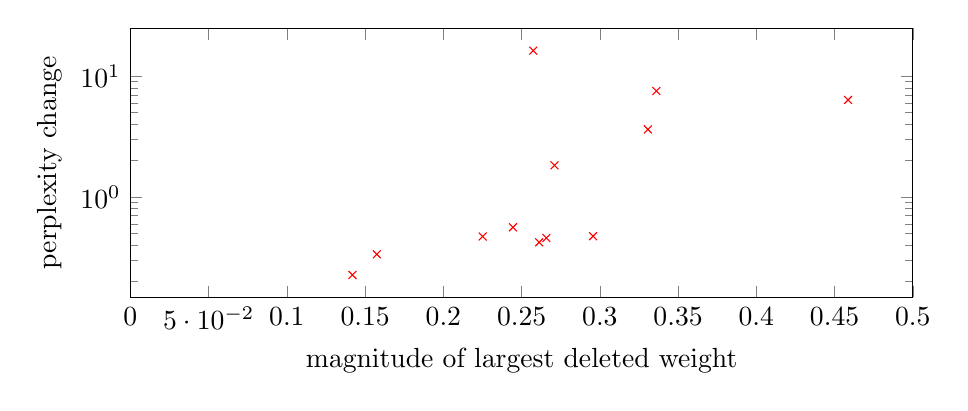
\begin{tikzpicture}
\begin{semilogyaxis}[
width=0.95\columnwidth,
height=5cm,
xlabel={magnitude of largest deleted weight}, 
ylabel={perplexity change},
xmin=0,
xmax=0.5,
]
\addplot[
only marks,
color=red,
mark=x,
]
table[row sep=crcr]
{
0.22513		0.471137\\
0.244492		0.561763\\
0.270999		1.829927\\
0.330704		3.628541\\
0.261247		0.422055\\
0.265832		0.457759\\
0.295644		0.473893\\
0.336088		7.545939\\
0.458583		6.362093\\
0.257479		16.277336\\
0.157486		0.335614\\
0.14194		0.226382\\
};
\end{semilogyaxis}
\end{tikzpicture}
\caption[Magnitude of largest deleted weight vs. perplexity change]{Magnitude of largest deleted weight vs. perplexity change, for the 12
different weight classes when pruning 90\% of parameters by class-uniform
pruning.}
\label{fig:scatter}
\end{figure}

\subsubsection{Pruning and retraining}
\label{subsec:effect}


Pruning has an immediate negative impact on performance (as measured by BLEU) that is exponential in pruning percentage; this is demonstrated by the blue line in Figure \ref{fig:main_results}.
However I find that up to about 40\% pruning, performance is mostly unaffected, indicating a large amount of redundancy and over-parameterization in NMT.

I now consider the effect of retraining pruned models.
The orange line in Figure \ref{fig:main_results} shows that after retraining the pruned models, baseline performance (20.48 BLEU) is both recovered and improved upon, up to 80\% pruning (20.91 BLEU), with only a small performance loss at 90\% pruning (20.13 BLEU).
This may seem surprising, as I might not expect a sparse model to significantly out-perform a model with five times as many parameters.
There are several possible explanations, two of which are given below.
\begin{figure}
\centering
% !TEX root = acl2016.tex

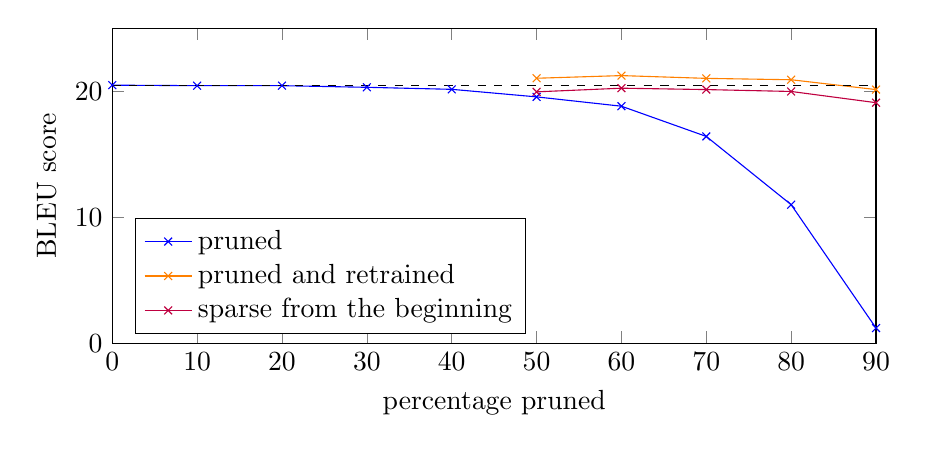
\begin{tikzpicture}

\begin{axis}[%
width=0.8\columnwidth,
height=4cm,
scale only axis,
xmin=0,
xmax=90,
xtick={0,10, 20, 30, 40, 50, 60, 70, 80, 90},
xlabel={percentage pruned},
ymin=0,
ymax=25,
yminorticks=true,
ylabel={BLEU score},
axis background/.style={fill=white},
legend pos = south west,
legend cell align=left,
]
\addplot [color=blue,solid,mark=x,mark options={solid}]
  table[row sep=crcr]{%
  0	20.48\\
10	20.44\\
20	20.44\\
30	20.31\\
40	20.15\\
50	19.55\\
60	18.81\\
70	16.41\\
80	10.99\\
90	1.2\\
};
\addlegendentry{pruned}

\addplot [color=orange,solid,mark=x,mark options={solid}]
  table[row sep=crcr]{%
50	21.03\\
60	21.24\\
70	21.02\\
80	20.91\\
90	20.13\\
};
\addlegendentry{pruned and retrained}

\addplot [color=purple,solid,mark=x,mark options={solid}]
  table[row sep=crcr]{%
50	19.95\\
60	20.24\\
70	20.13\\
80	19.98\\
90	19.09\\
};
\addlegendentry{sparse from the beginning}

\addplot [color=black,dashed]
  table[row sep=crcr]{%
0	20.48\\
90	20.48\\
};
\end{axis}
\end{tikzpicture}%
\caption[Performance of pruned models]{Performance of pruned models (a) after pruning, (b) after pruning and
retraining, and (c) when trained with sparsity structure from the outset (see
Section \ref{subsec:sparse}).}
\label{fig:main_results}
\end{figure}

Firstly, I found that the less-pruned models perform better on the training set than the validation set, whereas the more-pruned models have closer performance on the two sets. 
This indicates that pruning has a regularizing effect on the retraining phase, though clearly more is not always better, as the 50\% pruned and retrained model has better validation set performance than the 90\% pruned and retrained model.
Nonetheless, this regularization effect may explain why the pruned and retrained models outperform the baseline.
\begin{figure}[tbh]
\centering
% !TEX root = acl2016.tex

\begin{tikzpicture}

\begin{axis}[%
width=0.8\columnwidth,
height=4cm,
scale only axis,
xmin=0,
xmax=540000,
%xtick={},
xlabel={training iterations},
ymin=1,
ymax=8,
yminorticks=true,
ylabel={loss},
axis background/.style={fill=white},
%legend pos = south west,
%legend cell align=left
]

\addplot [color=black,dotted]
  table[row sep=crcr]{%
0	2.27\\
540000	2.27\\
};

\addplot [color=black,dotted]
  table[row sep=crcr]{%
405000	0\\
405000	8\\
};

\addplot [color=blue,solid,mark options={solid}]
  table[row sep=crcr]{%
5000	6.89\\
10000	5.91\\
15000	5.34\\
20000	4.88\\
25000	4.35\\
30000	3.9\\
35000	3.66\\
40000	3.61\\
45000	3.55\\
50000	3.5\\
55000	3.43\\
60000	3.3\\
65000	3.16\\
70000	3.07\\
75000	3.06\\
80000	3.05\\
85000	3.04\\
90000	3.01\\
95000	2.94\\
100000	2.86\\
105000	2.82\\
110000	2.82\\
115000	2.82\\
120000	2.81\\
125000	2.8\\
130000	2.75\\
135000	2.7\\
140000	2.67\\
145000	2.67\\
150000	2.67\\
155000	2.67\\
160000	2.66\\
165000	2.63\\
170000	2.59\\
175000	2.57\\
180000	2.57\\
185000	2.57\\
190000	2.57\\
195000	2.57\\
200000	2.54\\
205000	2.51\\
210000	2.5\\
215000	2.5\\
220000	2.5\\
225000	2.5\\
230000	2.5\\
235000	2.48\\
240000	2.45\\
245000	2.44\\
250000	2.44\\
255000	2.44\\
260000	2.44\\
265000	2.44\\
270000	2.42\\
275000	2.4\\
280000	2.39\\
285000	2.39\\
290000	2.4\\
295000	2.4\\
300000	2.4\\
305000	2.38\\
310000	2.36\\
315000	2.35\\
320000	2.35\\
325000	2.36\\
330000	2.36\\
335000	2.35\\
340000	2.34\\
345000	2.32\\
350000	2.31\\
355000	2.31\\
360000	2.31\\
365000	2.31\\
370000	2.31\\
375000	2.29\\
380000	2.28\\
385000	2.27\\
390000	2.27\\
395000	2.27\\
400000	2.27\\
405000	2.27\\
410000	2.53\\
415000	2.52\\
420000	2.48\\
425000	2.42\\
430000	2.22\\
435000	2.05\\
440000	1.99\\
445000	2.04\\
450000	2.08\\
455000	2.11\\
460000	2.12\\
465000	2.06\\
470000	1.99\\
475000	1.96\\
480000	1.99\\
485000	2.02\\
490000	2.03\\
495000	2.04\\
500000	2.01\\
505000	1.96\\
510000	1.95\\
515000	1.97\\
520000	1.98\\
525000	2\\
530000	2\\
535000	1.98\\
540000	1.95\\
};

\end{axis}
\end{tikzpicture}%
\caption[Validation set losses during training, pruning and retraining]{The validation set loss during training, pruning and retraining. The vertical dotted line marks the point when 80\% of the parameters are pruned. The horizontal dotted line marks the best performance of the unpruned baseline.}

\label{fig:loss_curve}
\end{figure}

\begin{figure*}
\centering
\includegraphics[width=\textwidth]{img/6-2_redundancy_good} %trim = 0mm 130mm 300mm 0mm, clip, 
\caption[Graphical representation of the location of small weights]{Graphical representation of the location of small weights in various parts of the model. 
Black pixels represent weights with absolute size in the bottom 80\%; white pixels represent those with absolute size in the top 20\%.
Equivalently, these pictures illustrate which parameters remain after pruning 80\% using my class-blind pruning scheme.
}
\label{fig:redundancy_location}
\end{figure*}



Alternatively, pruning may serve as a means to escape a local optimum. 
Figure \ref{fig:loss_curve} shows the loss function over time during the training, pruning and retraining process.
During the original training process, the loss curve flattens out and seems to converge (note that I use early stopping to obtain my baseline model, so the original model was trained for longer than shown in Figure \ref{fig:loss_curve}).
Pruning causes an immediate increase in the loss function, but enables further gradient descent, allowing the retraining process to find a new, better local optimum.
It seems that the disruption caused by pruning is beneficial in the long-run.

\subsubsection{Starting with sparse models}
\label{subsec:sparse}
The favorable performance of the pruned and retrained models raises the question: can I get a shortcut to this performance by \emph{starting} with sparse models?
That is, rather than train, prune, and retrain, what if I simply prune then train?
To test this, I took the sparsity structure of my 50\%--90\% pruned models, and trained completely new models with the same sparsity structure.
The purple line in Figure \ref{fig:main_results} shows that the `sparse from the beginning' models do not perform as well as the pruned and retrained models, but they do come close to the baseline performance.
This shows that while the sparsity structure alone contains useful information about redundancy and can therefore produce a competitive compressed model, it is important to interleave pruning with training.

Though my method involves just one pruning stage, other pruning methods interleave pruning with training more closely by including several iterations \cite{collins2014memory,han2015learning}.
I expect that implementing this for NMT would likely result in further compression and performance improvements.



\subsubsection{Storage size}
The original unpruned model (a MATLAB file) has size 782MB.
The 80\% pruned and retrained model is 272MB, which is a 65.2\% reduction.
In this work I focus on compression in terms of number of parameters rather than storage size, because it is invariant across implementations.

\subsubsection{Distribution of redundancy in NMT}
\label{subsubsec:redundancy}

I visualize in Figure~\ref{fig:redundancy_location} the redundancy structore of
my NMT baseline model.
{\it Black} pixels represent weights near to zero (those that can be pruned); {\it white} pixels represent larger ones.
First I consider the embedding weight matrices, whose columns correspond to words in the vocabulary.
Unsurprisingly, in Figure \ref{fig:redundancy_location}, I see that the parameters corresponding to the less common words are more dispensable.
In fact, at the 80\% pruning rate, for 100 uncommon source words and 1194
uncommon target words, I delete \emph{all} parameters corresponding to that word.
This is not quite the same as removing the word from the vocabulary --- true out-of-vocabulary words are mapped to the embedding for the `unknown word' symbol, whereas these `pruned-out' words are mapped to a zero embedding.
However in the original unpruned model these uncommon words already had near-zero embeddings, indicating that the model was unable to learn sufficiently distinctive representations.

Returning to Figure \ref{fig:redundancy_location}, now look at the eight weight matrices for the source and target connections at each of the four layers.
Each matrix corresponds to the $4n \times 2n$ matrix $T_{4n,2n}$ in Equation (\ref{eqn:lstm_1}).
In all eight matrices, I observe --- as does \cite{lu2016learning} --- that the weights connecting to the input $\hat{h}$ are most crucial, followed by the input gate $i$, then the output gate $o$, then the forget gate $f$. 
This is particularly true of the lower layers, which focus primarily on the input $\hat{h}$. 
However for higher layers, especially on the target side, weights connecting to the gates are as important as those connecting to the input $\hat{h}$.
The gates represent the LSTM's ability to add to, delete from or retrieve information from the memory cell.
Figure \ref{fig:redundancy_location} therefore shows that these sophisticated memory cell abilities are most important at the \emph{end} of the NMT pipeline (the top layer of the decoder).
This is reasonable, as I expect higher-level features to be learned later in a deep learning pipeline.

I also observe that for lower layers, the feed-forward input is much more important than the recurrent input, whereas for higher layers the recurrent input becomes more important.
This makes sense: lower layers concentrate on the low-level information from the current word embedding (the feed-forward input), whereas higher layers make use of the higher-level representation of the sentence so far (the recurrent input).

Lastly, on close inspection, I notice several white diagonals emerging within
some subsquares of the matrices in Figure \ref{fig:redundancy_location},
indicating that even without initializing the weights to identity matrices
(as is sometimes done \cite{le2015simple}),
an identity-like weight matrix is learned. At higher pruning percentages, these diagonals become more pronounced.

\subsection{Generalizability of my results}
To test the generalizability of my results, I also test my pruning approach
on a smaller, non-state-of-the-art NMT model trained on the WIT3 Vietnamese-English 
dataset \cite{iwslt15}, which consists of 133,000 sentence pairs.
This model is effectively a scaled-down version of the state-of-the-art model in \cite{luong15attn},
with fewer layers, smaller vocabulary size, smaller hidden layer size, no attention mechanism,
and about 11\% as many parameters in total.
It achieves a BLEU score of 9.61 on the validation set.

Although this model and its training set are on a different scale to my main model, 
and the language pair is different, 
I found very similar results. 
For this model, it is possible to prune 60\% of parameters with no immediate performance loss,
and with retraining it is possible to prune 90\%, and regain original performance.
My main observations from Section \ref{subsubsec:exp_schemes} %to \ref{subsubsec:redundancy}
are also replicated; in particular, class-blind pruning is most successful,
`sparse from the beginning' models are less successful than pruned and retrained models,
and I observe the same patterns as seen in Figure \ref{fig:redundancy_location}.


